% "{'chapitre':'slci_multiphy','classe':('PSI'),'type':('application'),'titre':'Direction automatique découplée', 'source':'Banque PT - SI A 2017','comp':['B2-02',],'corrige':True }"
\setchapterimage{fig_00.jpg}
\chapter*{Application \arabic{cptApplication} \\ 
Direction automatique découplée -- \ifprof Corrigé \else Sujet \fi}

\addcontentsline{toc}{section}{Application \arabic{cptApplication} : Direction automatique découplée  -- \ifprof Corrigé \else Sujet \fi}

\iflivret \stepcounter{cptApplication} \else
\ifprof  \stepcounter{cptApplication} \else \fi
\fi
\setcounter{question}{0}

\marginnote{Banque PT -- SI A 2017}
\marginnote{\UPSTIcompetence[2]{B2-02}}
\begin{marginfigure}
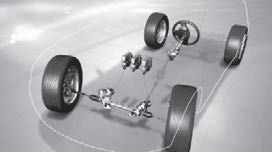
\includegraphics[width=\linewidth]{fig_01_b}
\end{marginfigure}


\ifprof
\else
Depuis maintenant de nombreuses années, les commandes de vol d'avions sont passées d'une
technologie purement mécanique à la technologie par fil (Fly by Wire). Le secteur automobile suit cette
tendance qui présente de nombreux avantages. C'est le système de direction par fil (Steer by Wire), encore nommé direction découplée, qui fait l'objet de l'étude proposée.


La \autoref{fig_09} donne une vue de cette unité sous la forme d'une maquette numérique à laquelle est
associé le schéma cinématique qui servira de base à l'étude mécanique.

\begin{figure}[H]
\centering
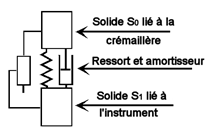
\includegraphics[width=.6\linewidth]{fig_09}

\caption{Unité de pilotage (chaîne d'énergie) et schéma cinématique  \label{fig_09}}
\end{figure}

L'unité de pilotage est constituée d'une chaîne d'énergie chargée de solliciter le volant par un
couple $C_{\text{mv}} \vect{x_v}$ qui résiste à l'action du conducteur $C_{c} \vect{x_v}$
quand celui-ci cherche à tourner le volant.

En effet, la simple dynamique du système mécanique de l'unité de pilotage ne donnerait pas au
conducteur la sensation de manier la direction d'une automobile. La composante $C_{\text{mv}}$ est donc élaborée pour que la dynamique du volant en termes d'inertie et de raideur soit équivalente à celle d'une direction conventionnelle optimisée selon le type de conduite visée.

La composante $C_{\text{mv}}$ est élaborée à partir de la consigne d'angle du volant $C_{\text{v\_ref}}$, transmise par le
générateur de consigne intégré au contrôleur de modèles, et de la composante $C_c$ du couple
conducteur.

Le modèle de la structure sous la forme d'un schéma bloc décrivant le comportement asservi de cette
unité est donné \autoref{fig_10}. On précise que la variable d'entrée est $\theta_{\text{v\_ref}}(p)$, que la variable de sortie est $\theta_{v}(p)$ et que la variable $C_c(p)$ est considérée comme une perturbation. Un signal de commande $U_{\text{mv}}(p)$ pilote la motorisation.



\begin{figure}[H]
\centering
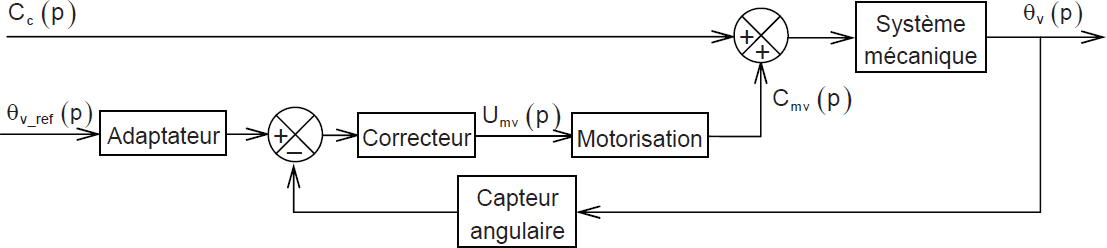
\includegraphics[width=\linewidth]{fig_10}

\caption{Unité de pilotage (chaîne d'énergie) et schéma cinématique  \label{fig_10}}
\end{figure}

Un modèle acausal de cette structure dont certains composants ne sont pas reliés aux autres, est
donné sur le cahier réponses.

\fi

\question{Compléter ce modèle en traçant les liens manquants qui donneraient un modèle équivalent au
schéma bloc de la \autoref{fig_10}.}
\ifprof
\begin{corrige}
\begin{figure}[H]
\centering
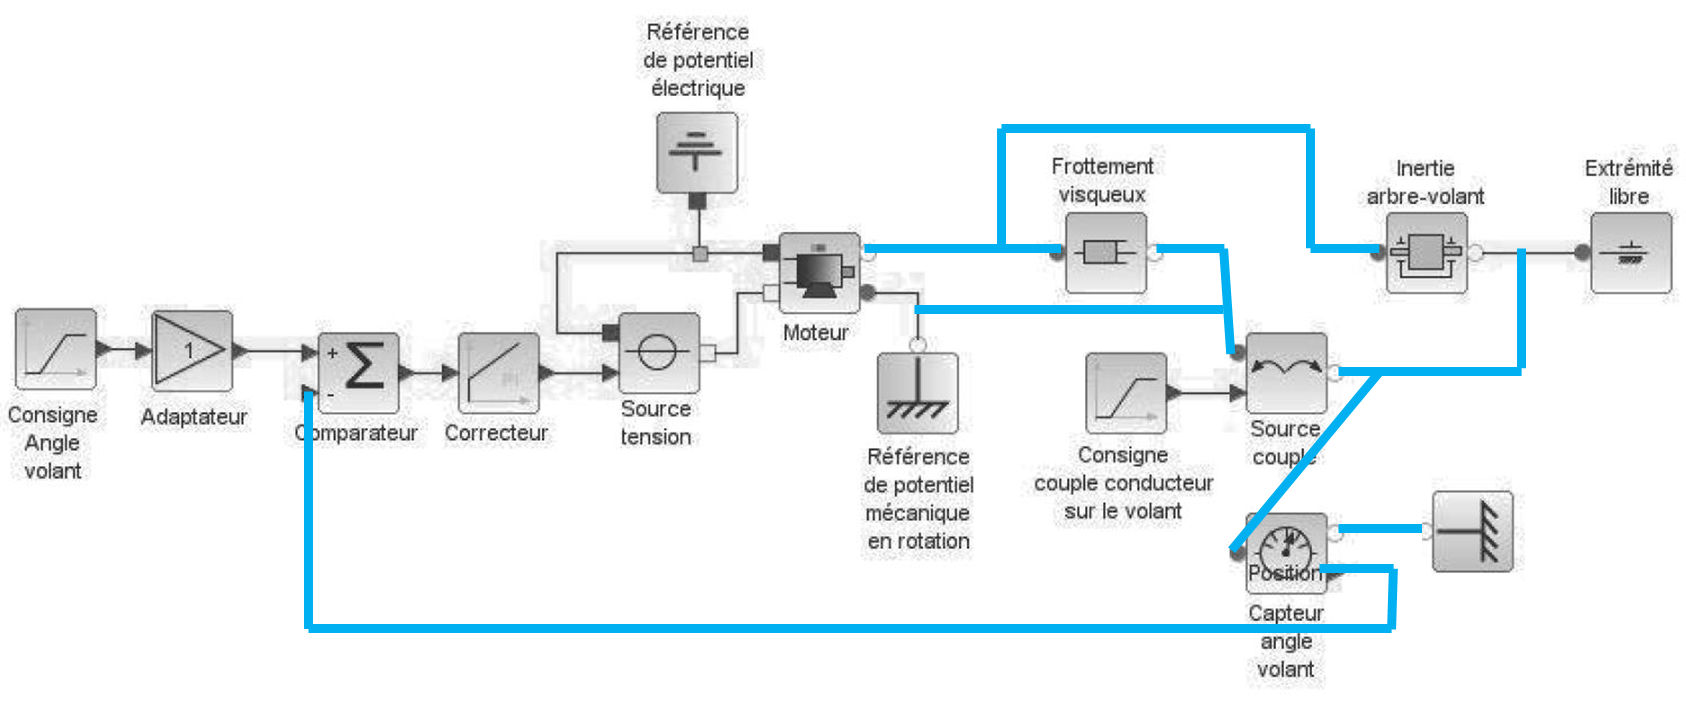
\includegraphics[width=.8\linewidth]{cor_02_bis}
\end{figure}
\end{corrige}
\else
\fi



\ifprof
\else
\begin{figure}[H]
\centering
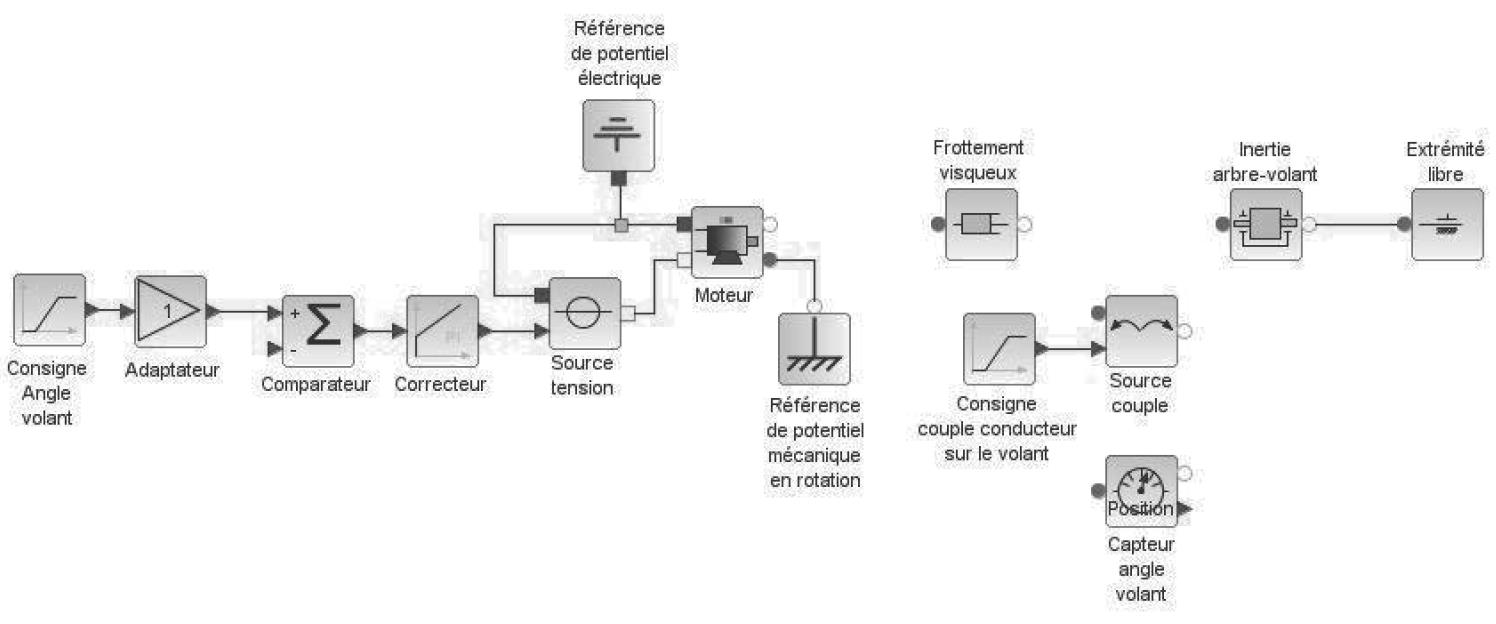
\includegraphics[width=\linewidth]{dr_01}
\end{figure}
\fi